\documentclass[aspectratio=169,xcolor=dvipsnames]{beamer}
\usetheme{Madrid}
\usepackage{ulem}
\usepackage{hyperref}
\usepackage{algorithm,algorithmic}
\usepackage{algorithm2e}
\usepackage{graphicx} % Allows including images
\makeatother
% The title
\title[Ant Q Algorithm \& Electric Vehicle Routing Problem]{Ant Q Algorithm}
\subtitle{and Electric Vehicle Routing problem}

\author[Tan Pham Ngoc] {Tan Pham Ngoc}
\institute[UIT] % Your institution may be shorthand to save space
{
    % Your institution for the title page
    Faculty of Computer Science \\
    University of Information Technology, VNU HCM 
    \vskip 3pt
}
\date{March 23, 2021} % Date, can be changed to a custom date


%----------------------------------------------------------------------------------------
%	PRESENTATION SLIDES
%------------------------0----------------------------------------------------------------

\begin{document}
%First slide
\begin{frame}
    \titlepage
\end{frame}

\begin{frame}
    \frametitle{Table of Contents}
    \tableofcontents[]
\end{frame}

%Table of contents
\AtBeginSection[]
{
  \begin{frame}
    \frametitle{Table of Contents}
    \tableofcontents[currentsection]
  \end{frame}
}

%Revise Q-Learning
\section{Revision on Q-Learning}
\begin{frame}{Q-Learning}
    \begin{figure}
        \centering
        
\includegraphics[scale = 0.04]{Life cycle.jpg}
        \label{fig:my_label}
    \end{figure}
\end{frame}

\begin{frame}{Q-Learning}
    \begin{figure}
        \centering
        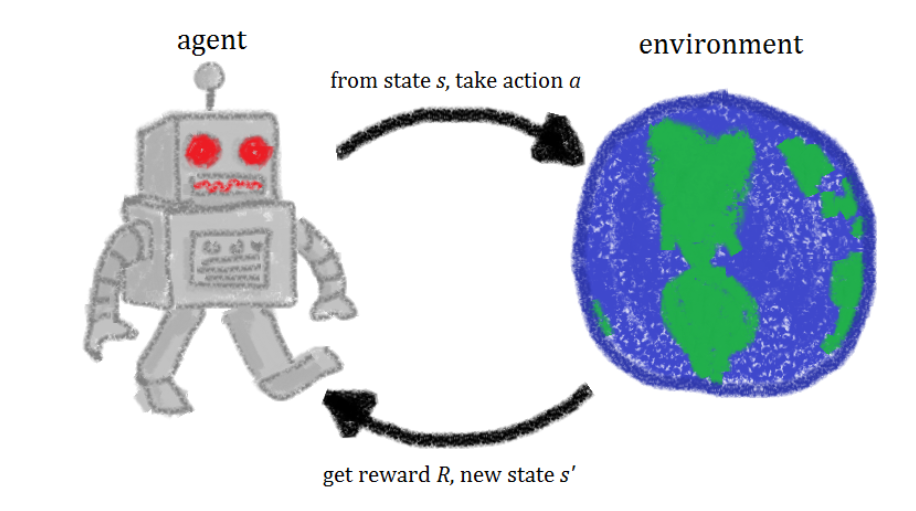
\includegraphics[scale = 0.5]{Q-learning description.png}
        \caption{Q-learning description}
        \label{fig:my_label}
    \end{figure}
\end{frame}

%Revise ACO
\section{Revise on Ant Colonization Optimization}
\begin{frame}{Ant Colonization Optimization}
    \begin{itemize}
        \item Marco Dorigo first introduced ACO in the early 90s
    \end{itemize}
\end{frame}

\begin{frame}{Ant Colonization Optimization}
    \begin{itemize}
        \item Marco Dorigo first introduced ACO in the early 90s
        \item The algorithm's development was inspired by the observation of the ant colonies
    \end{itemize}
\end{frame}

\begin{frame}{Ant Colonization Optimization}
    \begin{itemize}
        \item Marco Dorigo first introduced ACO in the early 90s
        \item The algorithm's development was inspired by the observation of the ant colonies
        \item The behavior that provided the inspiration for ACO is the ants' foraging behavior
    \end{itemize}
\end{frame}

\begin{frame}{Ant Colonization Optimization}
    \begin{figure}
        \centering
        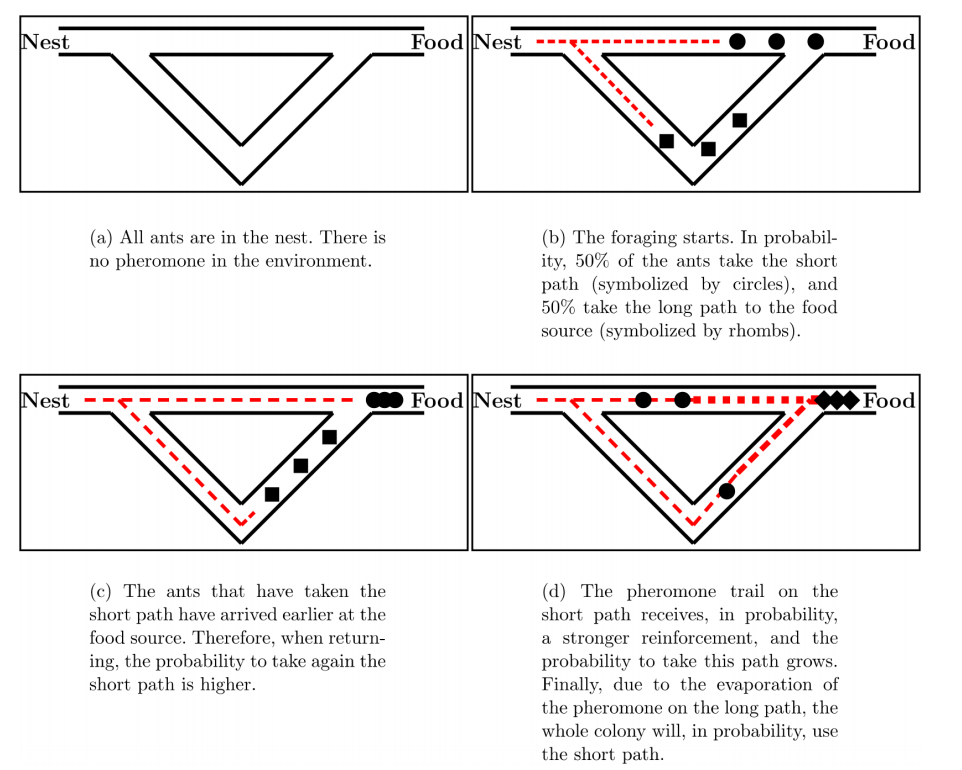
\includegraphics[scale = 0.40]{ACO description.png}
        \caption{ACO's brief description}
        \label{fig:my_label}
    \end{figure}
\end{frame}

%Brief introduction
\section{Brief introduction}
\begin{frame}{Introduction}
    \begin{itemize}
        \item Ant-Q is \alert{a family of algorithms} which present many similarities with Q-learning
    \end{itemize}
\end{frame}

\begin{frame}{Introduction}
    \begin{itemize}
        \item Ant-Q is \alert{a family of algorithms} which present many similarities with Q-learning
        \item It was inspired by the work on both the Dorigo et al, 1992, \textit{Ant System} and by Watkins, 1989, \textit{Q-Learning} 
    \end{itemize}
\end{frame}

\begin{frame}{Introduction}
    The core difference between Ant-Q and Q-learning:
\end{frame}

\begin{frame}{Introduction}
    The core difference between Ant-Q and Q-learning:
    \begin{itemize}
        \item Ant-Q uses \textit{\alert{a set of}} cooperating agents
    \end{itemize}
\end{frame}

\begin{frame}{Introduction}
    The core difference between Ant-Q and Q-learning:
    \begin{itemize}
        \item Ant-Q uses \textit{\alert{a set of}} cooperating agents
        \item These agents will cooperate exchanging information to each other in the form of \textit{\alert{AQ-values}}
    \end{itemize}
\end{frame}

\begin{frame}{Introduction}
    The core difference between Ant-Q and Q-learning:
    \begin{itemize}
        \item Ant-Q uses \textit{\alert{a set of}} cooperating agents
        \item These agents will cooperate exchanging information to each other in the form of \textit{\alert{AQ-values}}
        \item Over and above that, Ant-Q agents have \alert{memory}
    \end{itemize}
\end{frame}

%Mathematical view on Ant-Q
\section{A mathematical view on Ant-Q algorithm}
\begin{frame}{Mathematical view on Ant-Q}
    \begin{itemize}
        \item A graph $(N, E)$
    \end{itemize}
\end{frame}

\begin{frame}{Mathematical view on Ant-Q}
    \begin{itemize}
        \item A graph $(N, E)$
        \item A distance $d_{rs}$ for each pair of cities
    \end{itemize}
\end{frame}

\begin{frame}{Mathematical view on Ant-Q}
    \begin{itemize}
        \item A graph $(N, E)$
        \item A distance $d_{rs}$ for each pair of cities
        \begin{itemize}
            \item Symmetric: $d_{rs} = d_{sr}$
            \item Asymmetric: $d_{rs} \neq d_{sr}$
        \end{itemize}
    \end{itemize}
    
\end{frame}

\begin{frame}{Mathematical view on Ant-Q}
    Let denote:
\end{frame}

\begin{frame}{Mathematical view on Ant-Q}
    Let denote:
    \begin{itemize}
        \item $AQ(r,s)$ as \textit{Ant-Q value}: $AQ(r, s) \in \mathbb{R}^+$
    \end{itemize}
\end{frame}

\begin{frame}{Mathematical view on Ant-Q}
    Let denote:
    \begin{itemize}
        \item $AQ(r,s)$ as \textit{Ant-Q value}: $AQ(r, s) \in \mathbb{R}^+$
    \end{itemize}
    $\rightarrow$ The usefulness to move from city $r$ to city $s$
\end{frame}

\begin{frame}{Mathematical view on Ant-Q}
    Let denote:
    \begin{itemize}
        \item $AQ(r,s)$ as \textit{Ant-Q value}: $AQ(r, s) \in \mathbb{R}^+$
    \end{itemize}
    $\rightarrow$ The usefulness to move from city $r$ to city $s$
    \begin{itemize}
        \item $AQ'(r, s)$ as \textit{optimal Ant-Q value}
    \end{itemize}
\end{frame}

\begin{frame}{Mathematical view on Ant-Q}
    In the event of our graph:
    \begin{itemize}
        \item Symmetric:
        \item Asymmetric:
    \end{itemize}    
\end{frame}

\begin{frame}{Mathematical view on Ant-Q}
    In the event of our graph:
    \begin{itemize}
        \item Symmetric:
        \begin{center}
            $AQ(r, s) = AQ'(r, s)$
        \end{center}
        \item Asymmetric:
    \end{itemize}    
\end{frame}

\begin{frame}{Mathematical view on Ant-Q}
    In the event of our graph:
    \begin{itemize}
        \item Symmetric:
        \begin{center}
            $AQ(r, s) = AQ'(r, s)$
        \end{center}
        \item Asymmetric:
        \begin{center}
            $\left[AQ(r, s) = AQ'(r, s)\right] \lor \left[AQ(r, s) \neq AQ'(r, s)\right]$
            
        \end{center}
    \end{itemize}    
\end{frame}

\begin{frame}{Mathematical view on Ant-Q}
    Also, let define:
\end{frame}

\begin{frame}{Mathematical view on Ant-Q}
    Also, let define:
    \begin{itemize}
        \item $HE(r, s)$ as \textit{Heuristic values}
    \end{itemize}
\end{frame}

\begin{frame}{Mathematical view on Ant-Q}
    Also, let define:
    \begin{itemize}
        \item $HE(r, s)$ as \textit{Heuristic values}
        \begin{center}
            $HE(r, s) = \frac{1}{distance} = \frac{1}{d_{rs}}$
        \end{center}
    \end{itemize}
\end{frame}

\begin{frame}{Mathematical view on Ant-Q}
    Also, let define:
    \begin{itemize}
        \item $HE(r, s)$ as \textit{Heuristic values}
        \begin{center}
            $HE(r, s) = \frac{1}{distance} = \frac{1}{d_{rs}}$
        \end{center}
        $\rightarrow$ An heuristic evaluation of which move is better
    \end{itemize}
\end{frame}

\begin{frame}{Mathematical view on Ant-Q}
    Also, let define:
    \begin{itemize}
        \item $HE(r, s)$ as \textit{Heuristic values}
        \begin{center}
            $HE(r, s) = \frac{1}{distance} = \frac{1}{d_{rs}}$
        \end{center}
        $\rightarrow$ An heuristic evaluation of which move is better
        \item $k$ as the \textit{agent}, of which mission is to make tours
    \end{itemize}
\end{frame}

\begin{frame}{Mathematical view on Ant-Q}
    Also, let define:
    \begin{itemize}
        \item $HE(r, s)$ as \textit{Heuristic values}
        \begin{center}
            $HE(r, s) = \frac{1}{distance} = \frac{1}{d_{rs}}$
        \end{center}
        $\rightarrow$ An heuristic evaluation of which move is better
        \item $k$ as the \textit{agent}, of which mission is to make tours
        \item $J_k(r)$ as a list of cities \textit{to be visited} from the current city $r$
    \end{itemize}
\end{frame}

\begin{frame}
    \huge\centering With all of that, we have our \textit{\alert{action choice rule}}
\end{frame}

%Action choice rule
\subsection{Action choice rule}
\begin{frame}{Action choice rule}
    \textit{Action choice rule} can be understood easily as the rule for an agent $k$ in city $r$ move to city $s$:
\end{frame}

\begin{frame}{Action choice rule}
    \textit{Action choice rule} can be understood easily as the rule for an agent $k$ in city $r$ move to city $s$:
    \begin{equation*}
        s = \begin{cases}argmax_{u\in J_{k}(r)}\{\left[ AQ(r, u)\right]^\delta \cdot\left[HE(r, u)\right]^\beta\}&if\text{ } q\leq q_0\\S&otherwise\end{cases}
    \end{equation*}
\end{frame}

\begin{frame}{Action choice rule}
    \textit{Action choice rule} can be understood easily as the rule for an agent $k$ in city $r$ move to city $s$:
    \begin{equation*}
        s = \begin{cases}argmax_{u\in J_{k}(r)}\{\left[ AQ(r, u)\right]^\delta \cdot\left[HE(r, u)\right]^\beta\}&if\text{ } q\leq q_0\\S&otherwise\end{cases}
    \end{equation*}
    s.t.
    \begin{itemize}
        \item $\delta$, $\beta$: parameters weighing the relative importance of learning rate $AQ$ and $HE$
    \end{itemize}
\end{frame}

\begin{frame}{Action choice rule}
    \textit{Action choice rule} can be understood easily as the rule for an agent $k$ in city $r$ move to city $s$:
    \begin{equation*}
        s = \begin{cases}argmax_{u\in J_{k}(r)}\{\left[ AQ(r, u)\right]^\delta \cdot\left[HE(r, u)\right]^\beta\}&if\text{ } q\leq q_0\\S&otherwise\end{cases}
    \end{equation*}
    s.t.
    \begin{itemize}
        \item $\delta$, $\beta$: parameters weighing the relative importance of learning rate $AQ$ and $HE$
        \item $q$: uniformly distributed value in $\left[ 0; 1\right]$
        \item $q_0$: parameter following by the updated rule
    \end{itemize}
\end{frame}

\begin{frame}{Action choice rule}
    \textit{Action choice rule} can be understood easily as the rule for an agent $k$ in city $r$ move to city $s$:
    \begin{equation}
        s = \begin{cases}argmax_{u\in J_{k}(r)}\{\left[ AQ(r, u)\right]^\delta \cdot\left[HE(r, u)\right]^\beta\}&if\text{ } q\leq q_0\\S&otherwise\end{cases}
    \end{equation}
    s.t.
    \begin{itemize}
        \item $\delta$, $\beta$: parameters weighing the relative importance of learning rate $AQ$ and $HE$
        \item $q$: uniformly distributed value in $\left[ 0; 1\right]$
        \item $q_0$: parameter following by the updated rule
        \item $S$: a random variable selected according to a probability distribution given by function $AQ'(r, u)$ and $HE'(r, u)$ with $u \in J_k(r)$
    \end{itemize}
\end{frame}

\begin{frame}
    \huge\centering\textbf{Why multiply ?}
\end{frame}

\begin{frame}{Action choice rule}
    There are 3 main action choice rules:
    \begin{itemize}
        \item Pseudo-random
        \item Pseudo-random-proportional
        \item Random-proportional
    \end{itemize}
\end{frame}

\begin{frame}{Action choice rule}
    There are 3 main action choice rules:
    \begin{itemize}
        \item \textbf{Pseudo-random}
        \item Pseudo-random-proportional
        \item Random-proportional
    \end{itemize}
\end{frame}

\begin{frame}{Pseudo-random}
    The formula (1):
    \begin{equation*}
        s = \begin{cases}argmax_{u\in J_{k}(r)}\{\left[ AQ(r, u)\right]^\delta \cdot\left[HE(r, u)\right]^\beta\}&if\text{ } q\leq q_0\\S&otherwise\end{cases}
    \end{equation*}
    s.t. $S$, which is a random variable over the set $J_k(r)$, is selected according the uniform distribution
\end{frame}

\begin{frame}{Pseudo-random}
    The formula (1):
    \begin{equation*}
        s = \begin{cases}argmax_{u\in J_{k}(r)}\{\left[ AQ(r, u)\right]^\delta \cdot\left[HE(r, u)\right]^\beta\}&if\text{ } q\leq q_0\\S&otherwise\end{cases}
    \end{equation*}
    s.t.
    \textbf{$S$}, which is a random variable over the set $J_k(r)$, is selected according the uniform distribution\\
    \textbf{$\rightarrow$ Strongly resembles the action choice rule in Q-Learning}
\end{frame}

\begin{frame}{Action choice rule}
    There are 3 main action choice rules:
    \begin{itemize}
        \item Pseudo-random
        \item \textbf{Pseudo-random-proportional}
        \item Random-proportional
    \end{itemize}
\end{frame}

\begin{frame}{Pseudo-random-proportional}
    In the formula $(1)$, $S$ is a random variable over the set $N$, selected according to the distribution given below:
    \begin{equation*}
        p_k(r, s) = \begin{cases}\frac{\left[AQ\left(r, s\right)\right]^\delta \cdot\left[HE(r, s)\right]^\beta}{\sum_{u \in J_k(r)}\{\left[AQ\left(r, u\right)^\delta\cdot HE\left(r, u\right)^\beta\right]\}} &if \text{ }s\in J_k(r)\\0 &otherwise\end{cases}
    \end{equation*}
    $\rightarrow$ The probability with which an agent in city $r$ chooses the city $s$ to move to
\end{frame}

\begin{frame}{Action choice rule}
    There are 3 main action choice rules:
    \begin{itemize}
        \item Pseudo-random
        \item Pseudo-random-proportional
        \item \textbf{Random-proportional}
    \end{itemize}
\end{frame}

\begin{frame}{Random-proportional}
    \begin{itemize}
        \item Basically, this rule is the same as the pseudo-random-proportional in which $q_0 = 0$
        \item Specifically, the choice of the next city is always done by using random selection where edges are chosen with a probability distribution given by formula $(2)$
    \end{itemize}
    \begin{equation*}
        p_k(r, s) = \begin{cases}\frac{\left[AQ\left(r, s\right)\right]^\delta \cdot\left[HE(r, s)\right]^\beta}{\sum_{u \in J_k(r)}\{\left[AQ\left(r, u\right)^\delta\cdot HE\left(r, u\right)^\beta\right]\}} &if \text{ }s\in J_k(r)\\0 &otherwise\end{cases}
    \end{equation*}
\end{frame}

\begin{frame}{Random-proportional}
    \begin{itemize}
        \item Basically, this rule is the same as the pseudo-random-proportional in which $q_0 = 0$
        \item Specifically, the choice of the next city is always done by using random selection where edges are chosen with a probability distribution given by formula $(2)$
    \end{itemize}
    \begin{equation*}
        p_k(r, s) = \begin{cases}\frac{\left[AQ\left(r, s\right)\right]^\delta \cdot\left[HE(r, s)\right]^\beta}{\sum_{u \in J_k(r)}\{\left[AQ\left(r, u\right)^\delta\cdot HE\left(r, u\right)^\beta\right]\}} &if \text{ }s\in J_k(r)\\0 &otherwise\end{cases}
    \end{equation*}
    $\rightarrow$ The same as Ant-System
\end{frame}

%Agent's update rule
\subsection{Agent's update rule}
\begin{frame}{Agent's update rule}
\end{frame}

\begin{frame}{Agent's update rule}
    If the Q-value's update rule in DQN is shown as:
    \begin{equation*}
         Q_{\left(s,a\right)} \leftarrow \left( 1-\alpha \right) Q\left( s,a\right)  +\alpha {{\left(R_{t+1}+\gamma \max_{a^{^{\prime }}}Q\left( s^{\prime },a^{\prime }\right) \right) }}
    \end{equation*}
\end{frame}


\begin{frame}{Agent's update rule}
    Then the AQ-value in Ant-Q is updated as:
    \begin{equation*}
        AQ(r,s) \leftarrow (1 - \alpha)AQ(r, s) + \alpha\left(\Delta AQ(r, s) + \gamma \max_{z\in J_k(s)}AQ(s, z)\right)
    \end{equation*}
\end{frame}

\begin{frame}{Agent's update rule}
    Then the AQ-value in Ant-Q is updated as:
    \begin{equation*}
        AQ(r,s) \leftarrow (1 - \alpha)AQ(r, s) + \alpha\left(\Delta AQ(r, s) + \gamma \max_{z\in J_k(s)}AQ(s, z)\right)
    \end{equation*}
    in which:
\end{frame}

\begin{frame}{Agent's update rule}
    Then the AQ-value in Ant-Q is updated as:
    \begin{equation*}
        AQ(r,s) \leftarrow (1 - \alpha)AQ(r, s) + \alpha\left(\Delta AQ(r, s) + \gamma \max_{z\in J_k(s)}AQ(s, z)\right)
    \end{equation*}
    in which:
    \begin{itemize}
        \item $\alpha$: learning step 
        \item $\gamma$: discounted factor
    \end{itemize}
\end{frame}

\begin{frame}{Agent's update rule}
    Then the AQ-value in Ant-Q is updated as:
    \begin{equation*}
        AQ(r,s) \leftarrow (1 - \alpha)AQ(r, s) + \alpha\left(\Delta AQ(r, s) + \gamma \max_{z\in J_k(s)}AQ(s, z)\right)
    \end{equation*}
    in which:
    \begin{itemize}
        \item $\alpha$: learning step 
        \item $\gamma$: discounted factor
        \item $\Delta AQ(r, s)$: the delayed reinforcement
    \end{itemize}
\end{frame}

\begin{frame}{Agent's update rule}
    Then the AQ-value in Ant-Q is updated as:
    \begin{equation}
        AQ(r,s) \leftarrow (1 - \alpha)AQ(r, s) + \alpha\left(\Delta AQ(r, s) + \gamma \max_{z\in J_k(s)}AQ(s, z)\right)
    \end{equation}
    in which:
    \begin{itemize}
        \item $\alpha$: learning step 
        \item $\gamma$: discounted factor
        \item $\Delta AQ(r, s)$: the delayed reinforcement
    \end{itemize}
    $\Leftrightarrow$ The update rule $(3)$ is the same as the update rule in Q-learning, but we use the set $J_k(r)$ instead of the set of available actions in state $s$
\end{frame}

\begin{frame}
    \huge\centering\textbf{What is the delayed reinforcement ?}
\end{frame}
%The delayed reinforcement
\subsection{The delayed reinforcement}
\begin{frame}{The delayed reinforcement}
    \begin{itemize}
        \item Q-Learning's rewards 
    \end{itemize}
\end{frame}

\begin{frame}{The delayed reinforcement}
    \begin{itemize}
        \item Q-Learning's rewards $\rightarrow$ \textbf{\alert{Ant-Q's delayed reinforcement}}
    \end{itemize}
\end{frame}

\begin{frame}{The delayed reinforcement}
    \begin{itemize}
        \item Q-Learning's rewards $\rightarrow$ \textbf{\alert{Ant-Q's delayed reinforcement}}
        \item 2 types 
    \end{itemize}
\end{frame}

\begin{frame}{The delayed reinforcement}
    \begin{itemize}
        \item Q-Learning's rewards $\rightarrow$ \textbf{\alert{Ant-Q's delayed reinforcement}}
        \item 2 types 
        \begin{itemize}
            \item Global best
            \item Iteration best
        \end{itemize}
    \end{itemize}
\end{frame}

\begin{frame}{Global-best}
    \begin{equation*}
        \Delta AQ(r,s )= \begin{cases}\frac{W}{L_{k_{gb}}} &if\text{ }(r, s) \in \text {tour done by agent }k_{gb}\\0 &otherwise\end{cases}
    \end{equation*}
\end{frame}

\begin{frame}{Global-best}
    \begin{equation*}
        \Delta AQ(r,s )= \begin{cases}\frac{W}{L_{k_{gb}}} &if\text{ }(r, s) \in \text {tour done by agent }k_{gb}\\0 &otherwise\end{cases}
    \end{equation*}
    s.t.\\
    \begin{itemize}
        \item $W$ is often set to $10$
    \end{itemize}
\end{frame}

\begin{frame}{Global-best}
    \begin{equation}
        \Delta AQ(r,s )= \begin{cases}\frac{W}{L_{k_{gb}}} &if\text{ }(r, s) \in \text {tour done by agent }k_{gb}\\0 &otherwise\end{cases}
    \end{equation}
    s.t.\\
    \begin{itemize}
        \item $W$ is often set to $10$
        \item $L_{k_{gb}}$ is the tour made by the agent made the globally best tour from the beginning
    \end{itemize}
\end{frame}

\begin{frame}{Iteration-best}
    
\end{frame}

\begin{frame}{Iteration-best}
    \begin{equation*}
        \Delta AQ(r, s) = \begin{cases}\frac{W}{L_{k_{ib}}} &if \text{ } (r,s) \in \text{tour done by agent }k_{ib}\\0 &otherwise\end{cases}
    \end{equation*}
\end{frame}

\begin{frame}{Iteration-best}
    \begin{equation*}
        \Delta AQ(r, s) = \begin{cases}\frac{W}{L_{k_{ib}}} &if \text{ } (r,s) \in \text{tour done by agent }k_{ib}\\0 &otherwise\end{cases}
    \end{equation*}
    s.t.\\
    \begin{itemize}
        \item $k_{ib}$ is the agent who made best tour in the current iteration of the trial
    \end{itemize}
\end{frame}

%Difference between 2 algorithms
\begin{frame}
    \huge\centering\textbf{Ant-Q vs. Q-Learning}
\end{frame}

\begin{frame}{Ant-Q versus Q-Learning}
    
\end{frame}

%pseudocode
\begin{frame}
   \begin{figure}
        \centering
        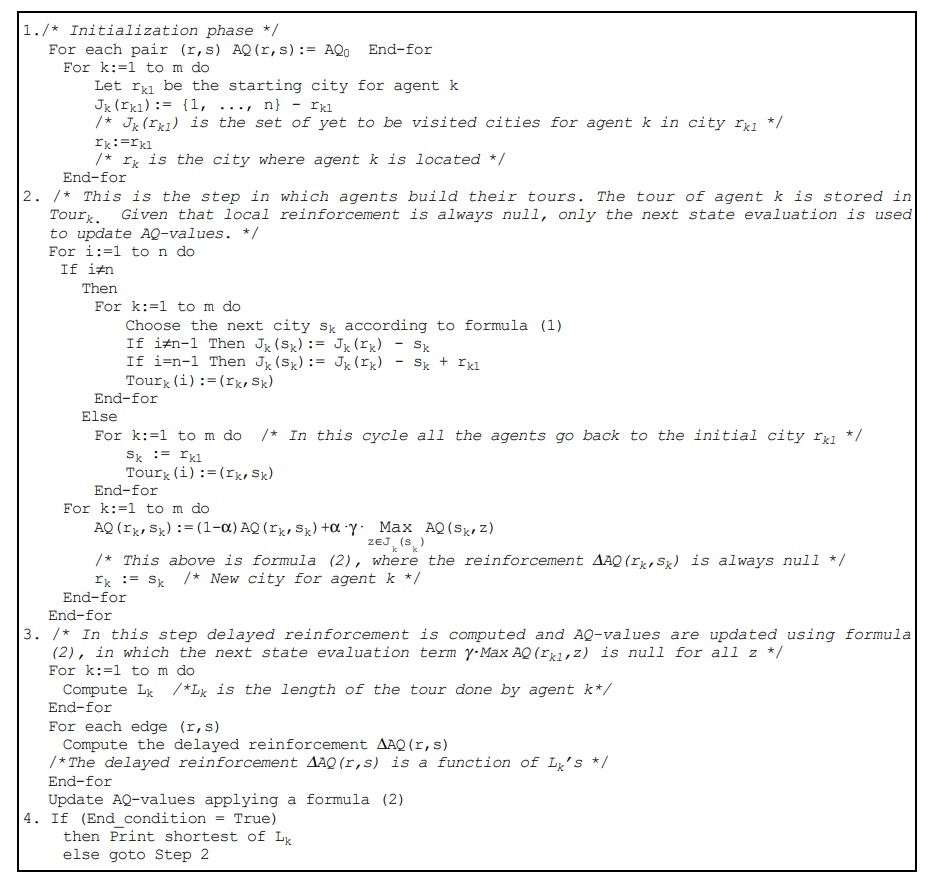
\includegraphics[scale = 0.40]{ACO pseudocode.png}
        \caption{ACO's brief description}
        \label{fig:my_label}
    \end{figure}
\end{frame}




\end{document}